% Sections 3 (efficiency) and 4 (failure mechanisms).
% Source: THEOREM_certificate_efficiency.md and ANALYSIS_T1_T3.md (project root).

\section{Efficiency of the certificate}\label{sec:analysis}

Proposition~\ref{prop:certificate} establishes the reliability of the feasible-pair certificate. This section examines its efficiency for the optimised
multiplier, in terms of the true displacement error, identifies conditions for bounded effectivity, and characterises exact certification. The results
apply to any feasible displacement approximation.

\subsection{An efficiency bound in the true error}

The key quantity is the complementarity of the \emph{exact} multiplier with the \emph{approximate} gap,
$\vlam\T\gh$. Since $\vlam\T\vg=0$ and $\gh=\vg-\mB\ve$,
\begin{equation}\label{eq:excess-identity}
  0\le\vlam\T\gh=-\vlam\T\mB\ve=-\sum_{i\in\Aplus}\lambda_i(\mB\ve)_i .
\end{equation}
For a row set $\Miss$, let $\vlam_{\Miss}$ denote $\vlam$ with entries outside $\Miss$ set to zero, and define
\begin{equation}\label{eq:intensity}
  m(\Miss):=\normKi{\mB\T\vlam_{\Miss}} .
\end{equation}
$m(\Aplus)=\normKi{\mB\T\vlam}=\normK{\vu-\mK^{-1}\vf}$ is the energy distance between the constrained and the unconstrained
solution, a measure of the contact intensity.

\begin{theorem}[efficiency]\label{thm:efficiency}
For every feasible $\uh$,
\begin{equation}\label{eq:efficiency}
  \normK{\ve}\ \le\ \Dstar(\lmr)\ \le\ \frac{2}{\sqrt3}\,\Phi(\lmr)^{1/2}\ \le\ \frac{2}{\sqrt3}\Big(s^2\normK{\ve}^2+\vlam\T\gh\Big)^{1/2},
\end{equation}
and $\vlam\T\gh\le m(\Aplus)\,\normK{\ve}$.
\end{theorem}
\begin{proof}
The first inequality is Proposition~\ref{prop:certificate} and the second is Lemma~\ref{lem:phi}. For the third, the exact multiplier
$\vlam\ge\boldsymbol 0$ is admissible in \eqref{eq:phi}, so $\Phi(\lmr)\le\Phi(\vlam)$. At $\vell=\vlam$ the residual is
$\vf+\mB\T\vlam-\mK\uh=\mK\ve$, and $\mK\preceq\gamma_X\mX$ is equivalent to $\mK\mX^{-1}\mK\preceq\gamma_X\mK$; hence
$\rhob(\vlam)^2=\ve\T\mK\mX^{-1}\mK\ve/\alpha_X\le s^2\normK{\ve}^2$, while $\eta(\vlam)=\vlam\T\gh$. The last claim follows from
\eqref{eq:excess-identity} and the Cauchy--Schwarz inequality in the $\mK^{-1}$/$\mK$ pairing.
\end{proof}

The first two inequalities in \eqref{eq:efficiency} are established results. For $\mX=\mK$, the identity
$\Phi(\vlam)=\normK{\ve}^2+\vlam\T\gh$ follows from the primal energy relation in Proposition~\ref{prop:gap}; its continuous counterpart
appears in \cite{bartels2025}. Theorem~\ref{thm:efficiency} extends this comparison to the computable surrogate-minimising multiplier,
introducing only the factor $2/\sqrt3$ and requiring no separate multiplier-error term.

Related studies establish efficiency estimates involving primal and multiplier errors \cite{veeser2001,braess2005,krause2015}, identify
contact-related contributions near free boundaries \cite{krause2015,weiss2010,braess2005}, and examine square-root differences between residual
bounds for reduced-basis approximations \cite{haasdonk2012}. Functional majorants for obstacle problems have also been minimised over
nonnegative multipliers \cite{repin2000,repin2007}, while primal--dual error identities identify contributions associated with contact-set mismatch
\cite{repin2018,bartels2025}. The present analysis focuses on the efficiency of the finite-dimensional surrogate-minimising certificate relative to
the primal error. Equivalent explicit statements of the efficiency bound, active-set consistency result, sharp half-rate example, and force-weighted
missed-row bound were not identified in the examined literature
\cite{haasdonk2012,zhang2016cr,zhang2016thesis,zhangs2020,bartels2025,ashby2024,veeser2001,braess2005,weiss2010,krause2015,nochetto2003,burkovska2015,benaceur2020,repin2000,repin2007,repin2018}.
This assessment is limited to the source versions examined, including preprints where published versions were unavailable.

\begin{remark}[inexact minimisation; sharper special case]\label{rem:inexact}
Any computed nonnegative multiplier $\tilde\vell$ remains admissible for certification. If
$\Phi(\tilde\vell)\le\Phi(\lmr)+\delta$, then
$\Dstar(\tilde\vell)\le\frac{2}{\sqrt3}(s^2\normK{\ve}^2+\vlam\T\gh+\delta)^{1/2}$.
If $\eta(\lmr)=0$, then $\Dstar(\lmr)=\rhob(\lmr)=\Phi(\lmr)^{1/2}$, and the factor $2/\sqrt3$ is unnecessary.
\end{remark}

\begin{corollary}[effectivity]\label{cor:effectivity}
Let $\mathrm{eff}:=\Dstar(\lmr)/\normK{\ve}$ for $\ve\ne\boldsymbol 0$.
\begin{enumerate}
\item[(a)] In general, $1\le\mathrm{eff}\le\frac{2}{\sqrt3}\big(s^2+m(\Aplus)/\normK{\ve}\big)^{1/2}$. Along a sequence with bounded $s$ and $m(\Aplus)$,
the certificate is therefore at worst of order $\normK{\ve}^{1/2}$; this upper rate need not be attained, but it is sharp in the
worst case (Proposition~\ref{prop:half-rate}).
\item[(b)] \emph{Active-set consistency.} If $\hat g_i=0$ for every $i\in\Aplus$, then $\vlam\T\gh=0$ and
\begin{equation}\label{eq:eff-consistent}
  1\le\mathrm{eff}\le\frac{2}{\sqrt3}\,s ;
\end{equation}
in particular $\mathrm{eff}\le2/\sqrt3\approx1.155$ for $\mX=\mK$, and $\mathrm{eff}\le\frac{2}{\sqrt3}\kappa(\mK)^{1/2}$ for $\mX=\mI$.
\item[(c)] If $\vlam\T\gh\le C\normK{\ve}^2$, then $\mathrm{eff}\le\frac{2}{\sqrt3}(s^2+C)^{1/2}$.
\end{enumerate}
\end{corollary}

Part (b) guarantees bounded effectivity when the approximation is in contact on every strictly active row. Uniformity across a family of problems
also requires bounded $s$. For $\mX=\mK(\vmu)$, $s=1$. With a positive affine stiffness decomposition and $\mX=\mK(\bar\vmu)$, the
coefficient ratios provide parameter-dependent bounds. For $\mX=\mI$, $s=\kappa(\mK)^{1/2}$ when exact extreme eigenvalues are used; this
factor may deteriorate under mesh refinement.

\begin{remark}[comparison with the primal--dual gap]\label{rem:gap-comparison}
Let $\mX=\mK$. The dual function $\mathcal D$ is strictly concave and maximised at $\vlam$, so
$\operatorname{arg\,min}_{\vell\ge0}G(\uh,\vell)=\vlam$ and
$\min_{\vell\ge0}G(\uh,\vell)=\frac12\normK{\ve}^2+\vlam\T\gh$. Consequently,
\[
  \Dstar(\vlam)\le\sqrt{2G(\uh,\vlam)}
  =\big(\normK{\ve}^2+2\vlam\T\gh\big)^{1/2}.
\]
This bound uses the exact multiplier, whose computation requires solving the full-order dual problem. By contrast,
Theorem~\ref{thm:efficiency} concerns the surrogate minimiser $\lmr$, which generally differs from $\vlam$ and need not minimise $\Dstar$.
The squared upper bounds are $\frac43(\normK{\ve}^2+\vlam\T\gh)$ and
$\normK{\ve}^2+2\vlam\T\gh$, respectively; the former is smaller when
$\vlam\T\gh>\frac12\normK{\ve}^2$. Thus, the efficiency result is a modest extension of the established gap identity, whereas the exactness and
failure-mechanism results require separate analysis.
\end{remark}

\subsection{S1 as a contact problem; exact certification}\label{sec:s1-contact}

For $\mX=\mK$ ($\alpha_X=1$), the surrogate-minimising multiplier solves a shifted contact problem. Define
$\vu_f:=\mK^{-1}\vf$ and $\mathbf H:=\mB\mK^{-1}\mB\T$, which is symmetric positive definite.

\begin{proposition}[S1 is a shifted contact problem]\label{prop:shifted}
Let $\mX=\mK$ and let $\uh$ be feasible. Then $\lmr$ solves
\begin{equation}\label{eq:shifted-lcp}
  \vell\ge\boldsymbol 0,\qquad \mathbf H\vell+\mB\vu_f-\vc'\ge\boldsymbol 0,\qquad \vell\T\big(\mathbf H\vell+\mB\vu_f-\vc'\big)=0,\qquad
  \vc':=\vc+\tfrac12\gh ,
\end{equation}
that is, $(\vu',\lmr)$ with $\vu':=\mK^{-1}(\vf+\mB\T\lmr)$ is the solution of the contact problem \eqref{eq:fom} with obstacle $\vc'$.
Moreover $\rhob(\lmr)=\normK{\uh-\vu'}$, the displacement $\uh$ is feasible for the problem with obstacle $\vc'$, and $\vu'$ is feasible for the
original problem.
\end{proposition}
\begin{proof}
$\nabla\Phi(\vell)=2\mB\mK^{-1}(\vf+\mB\T\vell-\mK\uh)+\gh=2(\mathbf H\vell+\mB\vu_f-\mB\uh)+\gh=2(\mathbf H\vell+\mB\vu_f-\vc-\tfrac12\gh)$, because $\mB\uh=\vc+\gh$.
$\Phi$ is strictly convex, so $\lmr$ is characterised by $\vell\ge\boldsymbol 0$, $\nabla\Phi\ge\boldsymbol 0$, $\vell\T\nabla\Phi=0$, which are \eqref{eq:shifted-lcp}; these are the
optimality conditions of \eqref{eq:fom} with obstacle $\vc'$, whose solution is unique. Then $\vf+\mB\T\lmr-\mK\uh=\mK(\vu'-\uh)$ gives
$\rhob(\lmr)=\normK{\uh-\vu'}$. Finally $\mB\uh=\vc+\gh\ge\vc'$ and $\mB\vu'\ge\vc'\ge\vc$.
\end{proof}

\begin{corollary}[exact certification]\label{cor:exact}
Let $\mX=\mK$ and $\boldsymbol 0\le\gh\le2\vg$ componentwise (in particular, $\hat g_i=0$ wherever $g_i=0$, so $\uh$ is in contact on the whole
contact set, and open rows are at most twice as open as in the exact solution). Then $\lmr=\vlam$, $\vu'=\vu$, and
\begin{equation}\label{eq:exact}
  \Dstar(\lmr)=\normK{\ve}.
\end{equation}
Conversely, for $\mX=\mK$ and feasible $\uh$, $\lmr=\vlam$ implies $\boldsymbol 0\le\gh\le2\vg$. Hence $\lmr=\vlam$ if and only if $\boldsymbol 0\le\gh\le2\vg$.
\end{corollary}
\begin{proof}
$(\vu,\vlam)$ satisfies \eqref{eq:shifted-lcp}: $\mB\vu-\vc'=\vg-\tfrac12\gh\ge\boldsymbol 0$, and $\lambda_i>0$ implies $g_i=0$, hence $\hat g_i=0$ and
$(\vg-\frac12\gh)_i=0$. By uniqueness, $\lmr=\vlam$ and $\vu'=\vu$. Then $\rhob(\lmr)=\normK{\uh-\vu}=\normK{\ve}$ and $\vlam\T\gh=0$.
Conversely, if $\lmr=\vlam$, then $\vu'=\mK^{-1}(\vf+\mB\T\vlam)=\vu$, and \eqref{eq:shifted-lcp} gives $\vg-\frac12\gh=\mB\vu-\vc'\ge\boldsymbol 0$, that is $\gh\le2\vg$; together with $\gh\ge\boldsymbol 0$ this is the condition.
(The converse implication from exact certificate effectivity to exact multiplier recovery is not asserted.)
\end{proof}

Corollary~\ref{cor:exact} strengthens the bounded-effectivity result for $\mX=\mK$ to exact certification. Because the condition involves the
unknown exact gap, it provides an analytical characterisation rather than an online test. Thus, reliability holds for any feasible approximation,
active-set consistency ensures bounded effectivity, and the stronger gap condition yields exact certification.

The shifted-contact interpretation also applies to a multiplier restricted to a support $S$. The corresponding displacement $\vu'_S$ satisfies only
the shifted constraints indexed by $S$ and may violate omitted constraints. Nevertheless, the certificate remains valid because $\uh$ is feasible
and $\lmr_S\ge0$, with residual $\rhob(\lmr_S)=\normK{\uh-\vu'_S}$. If $S$ omits a strictly active row, then $\vu'_S\ne\vu$; otherwise,
equilibrium and the injectivity of $\mB\T$ would imply $\lambda_i=0$ outside $S$, contradicting strict activity. This explains the restricted-support
certificate floor established below.

\section{Failure mechanisms}\label{sec:failure}

This section examines two limitations of certificate efficiency. The first arises when contact constraints that are strictly active in the exact
solution remain open in the approximation. The second results from excluding strictly active constraints from the multiplier support.

\subsection{The half rate cannot be removed by the multiplier}

\begin{proposition}[square-root degradation of the certificate family]\label{prop:half-rate}
Without active-set consistency, no multiplier restores the full rate in the worst case within the certificate \eqref{eq:certificate}; this is a property of this family, not a bound for every error estimator. Let $N=2$, $n_c=1$, $\mK=\mI$,
$\mB=[1\ \,0]$, $\vc=0$, $\vf=(-1,0)\T$ and $\mX=\mK$. The solution is $\vu=\boldsymbol 0$, $\lambda=1$, and the feasible approximation
$\uh=(\varepsilon,0)\T$, $\varepsilon>0$, has $\normK{\ve}=\varepsilon$. Then
\begin{equation}\label{eq:half-rate}
  \min_{\ell\ge0}\Dstar(\ell)=\sqrt{\varepsilon(1+\varepsilon)}\quad(\text{attained at }\ell=1+\varepsilon),\qquad
  \min_{\ell\ge0}\frac{\Dstar(\ell)}{\normK{\ve}}=\Big(\frac{1+\varepsilon}{\varepsilon}\Big)^{1/2}\to\infty .
\end{equation}
\end{proposition}
\begin{proof}
Here $\hat g=\varepsilon$, $\rhob(\ell)=|\ell-1-\varepsilon|$ and $\eta(\ell)=\ell\varepsilon$; write $\Delta=\Dstar(\ell)$, which satisfies $\Delta^2=\rhob\Delta+\ell\varepsilon$. At
$\ell=1+\varepsilon$, $\rhob=0$ and $\Delta=\sqrt{\varepsilon(1+\varepsilon)}$. If $\ell\ge1+\varepsilon$, then $\Delta^2\ge\ell\varepsilon\ge\varepsilon(1+\varepsilon)$. If $\ell<1+\varepsilon$, then
$\Delta^2=(1+\varepsilon)\Delta-\ell(\Delta-\varepsilon)$. For $\Delta\ge\varepsilon$ this gives $\Delta^2\ge(1+\varepsilon)\Delta-(1+\varepsilon)(\Delta-\varepsilon)=\varepsilon(1+\varepsilon)$; for $\Delta<\varepsilon$ it gives
$\Delta^2\ge(1+\varepsilon)\Delta$, i.e.\ $\Delta\ge1+\varepsilon>\varepsilon$, a contradiction.
\end{proof}

The square-root gap between residual bounds for variational inequalities was observed in \cite[Remark~4.5]{haasdonk2012}. This example
demonstrates that the degradation persists under unrestricted multiplier optimisation within the considered certificate family. It arises because
the approximation leaves open a contact constraint that is strictly active in the exact solution; it does not establish a limitation for other error
estimators.

\begin{figure}[t]
\centering
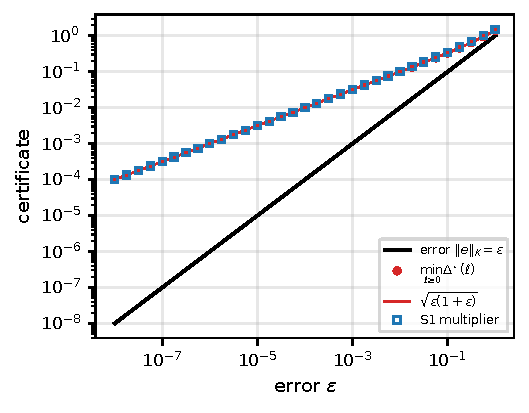
\includegraphics[width=0.62\linewidth]{figures/fig_halfrate}
\caption{The example of Proposition~\ref{prop:half-rate}. The error is $\varepsilon$ (slope $1$); the minimum of the certificate over all nonnegative multipliers,
computed numerically with the certificate code and compared with $\sqrt{\varepsilon(1+\varepsilon)}$, has slope $1/2$. The S1 multiplier, which in this example is
$\ell=1+\varepsilon/2$ and not the minimiser, gives a certificate that is visually indistinguishable from the minimum.}
\label{fig:half-rate}
\end{figure}

\subsection{Missed rows}

Corollary~\ref{cor:effectivity} covers the two extremes. For approximations that do not satisfy active-set consistency, the relevant complementarity contribution arises exclusively from strictly active
contact constraints that remain open in $\uh$.

\begin{theorem}[missed rows]\label{thm:missed}
Let $\Miss(\uh):=\{i\in\Aplus:\hat g_i>0\}$ be the rows of $\uh$ that are open although they carry a positive contact force in the
exact solution. Then
\begin{equation}\label{eq:missed}
  \vlam\T\gh=\sum_{i\in\Miss}\lambda_i\hat g_i=-\vlam_{\Miss}\T\mB\ve\le m(\Miss)\,\normK{\ve},
\end{equation}
and consequently
\begin{equation}\label{eq:missed-eff}
  \mathrm{eff}\le\frac{2}{\sqrt3}\Big(s^2+\frac{m(\Miss)}{\normK{\ve}}\Big)^{1/2}\le\frac{2}{\sqrt3}\Big(s+\sqrt{m(\Miss)/\normK{\ve}}\Big).
\end{equation}
\end{theorem}
\begin{proof}
In \eqref{eq:excess-identity} only rows with $\lambda_i>0$ and $\hat g_i>0$ contribute; on $\Aplus$, $\hat g_i=-(\mB\ve)_i$. The
bound follows from the Cauchy--Schwarz inequality, \eqref{eq:missed-eff} from Theorem~\ref{thm:efficiency} and
$\sqrt{a+b}\le\sqrt a+\sqrt b$.
\end{proof}

For $\Miss=\emptyset$, Theorem~\ref{thm:missed} recovers the active-set consistency bound. The bounds involving $m(\Miss)$ and
$m(\Aplus)$ are independent, since $m(\Miss)\le m(\Aplus)$ need not hold. In Proposition~\ref{prop:half-rate},
$\Miss=\{1\}$ and $m(\Miss)=1$, giving an upper bound proportional to $(\varepsilon^2+\varepsilon)^{1/2}$, within the factor
$2/\sqrt3$ of the exact minimum.

The energy-norm form \eqref{eq:missed} ignores how many rows are missed and how large their forces are. A localized
form makes this explicit and gives intermediate rates.

\begin{corollary}[localized form]\label{cor:localized}
With the notation of Theorem~\ref{thm:missed} (a maximum or norm over the empty set $\Miss=\emptyset$ is zero, and then $\vlam\T\gh=0$),
\begin{equation}\label{eq:localized}
  \vlam\T\gh\le\min\Big\{\norm{\vlam_{\Miss}}_2\,\norm{\gh_{\Miss}}_2,\ \norm{\vlam_{\Miss}}_1\max_{i\in\Miss}\hat g_i\Big\}.
\end{equation}
If, along a sequence of approximations, $\norm{\vlam_{\Miss}}_1\le C_\lambda\normK{\ve}^{a}$ for some $a\in[0,1]$ and
$\max_{\Miss}\hat g_i\le C_g\normK{\ve}$, then
\begin{equation}\label{eq:intermediate-rate}
  \Dstar(\lmr)\le\frac{2}{\sqrt3}\Big(s\,\normK{\ve}+(C_\lambda C_g)^{1/2}\normK{\ve}^{(1+a)/2}\Big).
\end{equation}
\end{corollary}
\begin{proof}
Hölder's inequality on the finite sum $\sum_{i\in\Miss}\lambda_i\hat g_i$, with exponents $(2,2)$ and $(1,\infty)$, then Theorem~\ref{thm:efficiency}. (The two bounds are separate; neither implies the other.)
\end{proof}

The exponent $a$ represents the assumed decay of contact forces on missed constraints, giving an upper rate of order
$\normK{\ve}^{(1+a)/2}$ when the constants remain bounded. This rate is not asserted to be sharp for every $a$. The gap condition holds with
$C_g=\max_i H_{ii}^{1/2}$, where $\mathbf H=\mB\mK^{-1}\mB\T$. Thus, the substantive additional assumption concerns the decay of
$\norm{\vlam_{\Miss}}_1$.

\subsection{Restricting the support of the multiplier}

The minimum-residual problem \eqref{eq:phi} has $n_c$ unknowns. For a row set $S$ let
$\lmr_S:=\operatorname{arg\,min}\{\Phi(\vell):\vell\ge\boldsymbol 0,\ \ell_i=0\text{ for }i\notin S\}$, and let $\mB_S$ denote the rows of $\mB$ in $S$ and
$S^c$ the complement.

\begin{theorem}[restricted support]\label{thm:support}
For every feasible $\uh$ and every $S$,
\begin{align}
  \Dstar(\lmr_S)&\le\frac{2}{\sqrt3}\Big(s^2\big(\normK{\ve}+m(S^c)\big)^2+\vlam\T\gh\Big)^{1/2},\label{eq:support-upper}\\
  \Dstar(\lmr_S)&\ge\frac{\sigma_S-\sqrt{\gamma_X}\,\normK{\ve}}{\sqrt{\alpha_X}},\qquad
  \sigma_S:=\min_{\vv\in\mathbb R^{|S|}}\normXi{\mB\T\vlam_{S^c}-\mB_S\T\vv}.\label{eq:support-lower}
\end{align}
Moreover $\sigma_S>0$ if and only if $\Aplus\not\subseteq S$.
\end{theorem}
\begin{proof}
The vector $\vlam_S$ is admissible, so $\Phi(\lmr_S)\le\Phi(\vlam_S)$. Its residual is $\mK\ve-\mB\T\vlam_{S^c}$, and
$\normXi{\vv}\le\sqrt{\gamma_X}\normKi{\vv}$ gives $\rhob(\vlam_S)\le s(\normK{\ve}+m(S^c))$; moreover $\vlam_S\T\gh\le\vlam\T\gh$. Lemma~\ref{lem:phi} yields
\eqref{eq:support-upper}. For \eqref{eq:support-lower}, any admissible $\vell$ has residual $\mK\ve-\mB\T(\vlam-\vell)$, so
$\sqrt{\alpha_X}\Dstar(\vell)\ge\normXi{\mB\T(\vlam-\vell)}-\normXi{\mK\ve}$; the first norm is at least $\sigma_S$ (drop the sign constraint) and
the second at most $\sqrt{\gamma_X}\normK{\ve}$. Finally, $\mB\T$ has full column rank, so $\mB\T\vlam_{S^c}\in\operatorname{range}\mB_S\T$ only if
$\vlam_{S^c}=\boldsymbol 0$.
\end{proof}

The quantity $\sigma_S$ depends on the exact multiplier and therefore provides an analytical diagnostic rather than an online support test. If
$S\supseteq\Aplus$, the restricted certificate satisfies the same efficiency bound as the unrestricted certificate. For a fixed problem and
support that omits a strictly active row,
\[
  \liminf_{\normK{\ve}\to0}\Dstar(\lmr_S)\ge\frac{\sigma_S}{\sqrt{\alpha_X}}>0.
\]
For varying problems or supports, a positive asymptotic floor requires $\sigma_S/\sqrt{\alpha_X}$ to remain bounded away from zero. Thus, missed
contact constraints in the displacement approximation may cause square-root degradation, whereas omitted active components in the multiplier support
may prevent certificate convergence. The gap-based support $S_t:=\{i:\hat g_i\le t\}$ contains $\Aplus$ whenever
$\norm{\mB\ve}_\infty\le t$.
